\documentclass[10pt,a4paper]{article}
\usepackage[utf8]{inputenc}
\usepackage[french]{babel}
\usepackage[T1]{fontenc}
\usepackage{amsmath}
\usepackage{amsfonts}
\usepackage{amssymb}
\usepackage{graphicx}
\usepackage{amsthm}
\usepackage{systeme}
\usepackage{stmaryrd}

\theoremstyle{definition}
\newtheorem{definition}{Définition}
\theoremstyle{definition}
\newtheorem{theorem}{Théorème}

\author{Della Bona Sarah, Dumez Erika}
\title{Introduction to neural ODE}
\begin{document}
\maketitle
 
 
\section{Ordinary Differential Equations}

\subsection{A reminder on ODE}

An ODE is a function that describes the changes of a function, $u$, through time. In this setting, time is a continuous variable and we don't know the real function, only its derivative.

\begin{definition}
Let $f: \Omega \subseteq \mathbb{R} \times \mathbb{R}^N \rightarrow \mathbb{R}^N$. 

A \textit{first order ODE} takes of the form:
\[
\partial_t u(t) = f(t,u(t)) \textbf{   (1)}
\]

\begin{itemize}
\item A \textit{solution} for (1) is a function $u : I \rightarrow \mathbb{R}^N$ where $I$ is an interval of $\mathbb{R}$ such that:
	\begin{itemize}
	\item u is derivable on I,
	\item $\forall t \in I, f(t, u(t)) \in \Omega$,
	\item $\forall t \in I, \partial_t u(t) = f(t, u(t))$
	\end{itemize}
\item An \textit{initial condition} (IC) is a condition of the type:
\[
u(t_0) = u_0
\]
where $(t_0, u_0) \in \Omega$ is fixed.
\end{itemize}
\item A \textit{Cauchy problem} is an ODE with IC
\[
\left \{
\begin{array}{rcl}
\partial_t u(t) & = & f(t, u(t)) \\
u(t_0) & = & u_0
\end{array}
\right.
\]
\end{definition}

\begin{definition}
A \textit{k-order ODE} is of the form:
\[
\partial^k_t v(t) = g(t, v(t), ... , \partial^{k-1}v(t))
\]
where 
   \begin{eqnarray}
   \nonumber
   v & : & I \rightarrow \mathbb{R}^N \\ 
   \nonumber
   g & : & \Theta \subseteq \mathbb{R} \times \mathbb{R}^N \times ... \times \mathbb{R}^N \rightarrow \mathbb{R}^N
   \end{eqnarray}
\end{definition}

It is not always possible to explicitly find a solution to a Cauchy problem, but we can compute a finite number of points $u_i \in \mathbb{R}^N$ which are close to the real solution. 

More precisely, let $T \in \mathbb{R}\\\{0\}$ such that the solution $u$ exists on $[t_0, t_0 + T]$ and let $n \in \mathbb{N}^{\geqslant 2}$. We are then looking for $(u_i)^n_{i=0}$ s.t. 
\[
u_i \approx u(t_i) \ \text{ where } t_0 < ... < t_n \in [t_0, t_0 + T]
\]

Let $h_i := t_{i+1} - t_i$, it is called the \textit{step}. To compute those $u_i$, we use \textit{1-step methods} such as Euler's method.

\subsection{Euler's method}

Euler's method is similar to a Taylor development, the idea is to compute $u(t_{i+1})$ using the following formula:\footnote{We consider that $ \forall i\ \{0,...,n\}, h_i = h$.}
\[
u(t_{i+1}) \approx u(t_i) + h . \partial u(t_i)
\]
where 
\[
\partial u(t_i) = f(t_i, u(t_i)).
\]

\section{Neural networks}

In a typical machine learning problem, you are given some input $x$ and you want to predict an output $y$. A \textit{neural network} can be used to solve such a problem. It consists of a series of layers. There are three types of layers :

\begin{itemize}
\item The \textit{input} layer
\item The \textit{output} layer
\item The \textit{hidden} layers
\end{itemize}

Each layer consist of a certain number of neurons. We give an input to the neurons of a layer, they do some calculus (non-linear activation function for example) and they give an output. Therefore, layers can be seen has matrix operations. 

The neurons of a layer are connected to the neurons of the next layer. Thanks to these connections, the output given by a neuron can be transmitted over the neural network. We begin by giving an input to the input layer, which transmits information to the first hidden layer (There isn't always an hidden layer in a neural network. In this case, the input layer is directly connected to the output layer). In turn, it transmit information to the next hidden layer and so on, until the output layer which give us the final output, the prediction. 

With a loss function, we can then determined the accuracy of the neural network and make it more accurate by changing the parameters. We are trying to find the optimal parameters which minimize this loss function. In order to do that, we use gradient descent.

We can see a neural network as a composite of functions, a function for each layer. That is because each layer uses an activation function on its input. Each layer introduces a little bit of error that propagate through the network.

\begin{center}
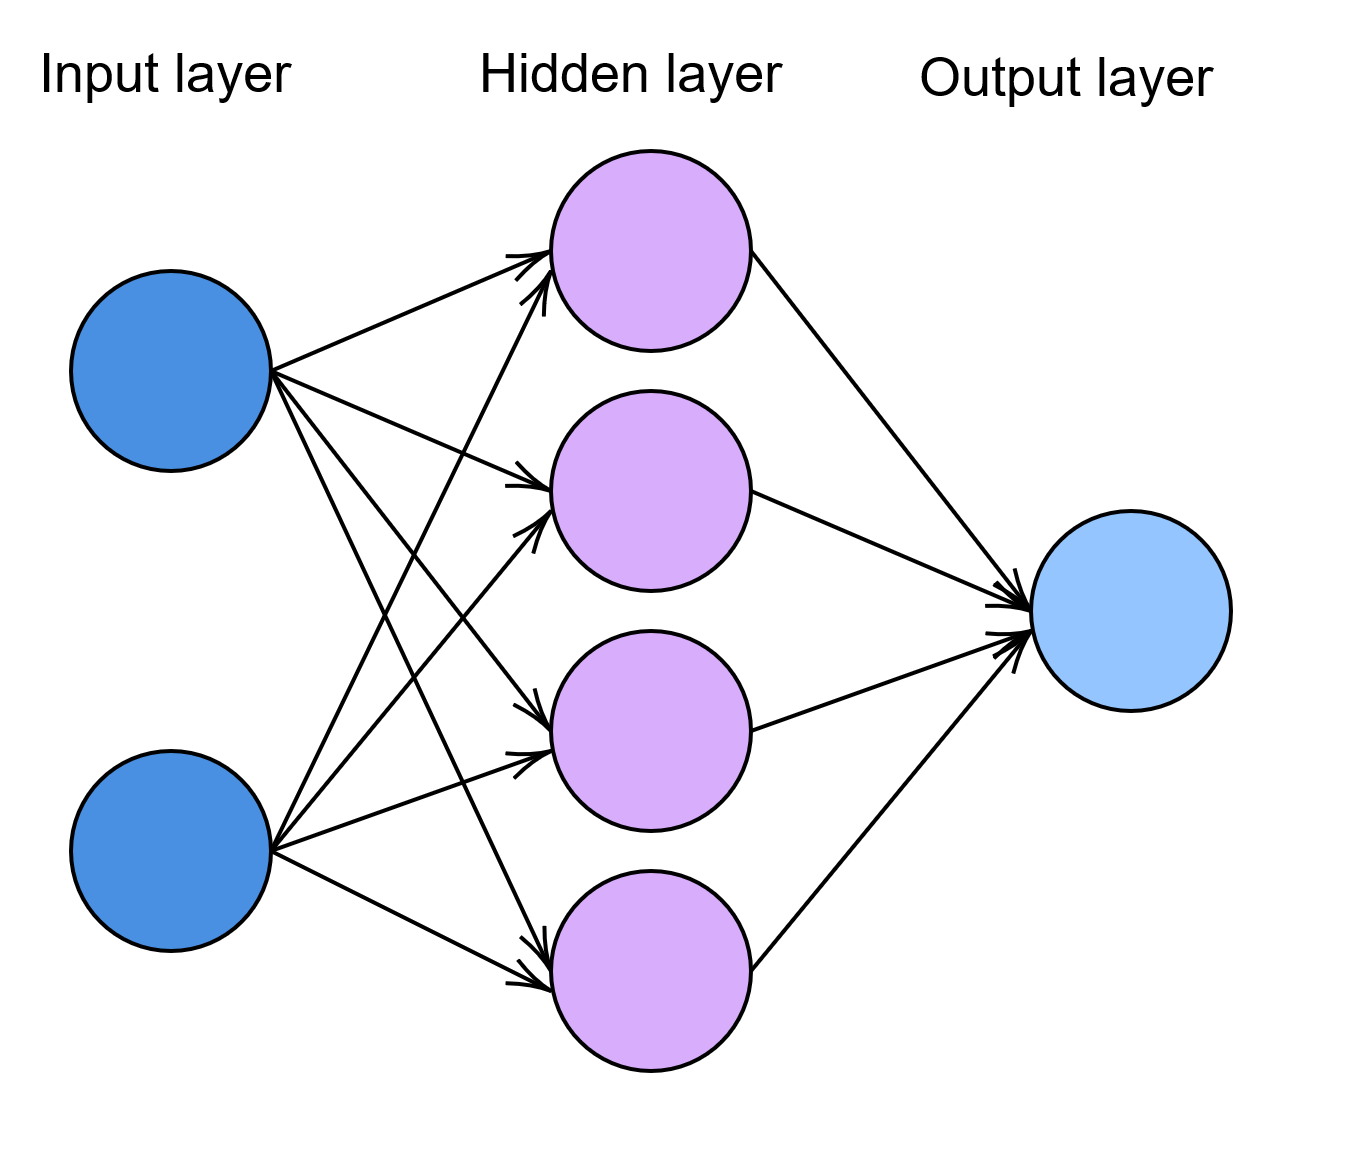
\includegraphics[scale=0.55]{nn.png}
\end{center}  

\subsection{Example} \label{2.1}

Let's consider a neural network, with one hidden layer, that takes a 2-dimensional input $x = (x_1, x_2)$, and gives a 2-dimensional output $y = (y_1,y_2)$. We can represent this network with the following equations:

   \begin{eqnarray}
   \nonumber
   z_i & = & \sum_{j=1}^2 w_{ij}^{(1)}x_j + b_i^{(1)} \text{ pour } i = 1,2 \\ 
   \nonumber
   h_i & = & \sigma (z_i) \text{ pour } i=1,2 \\
   \nonumber
   y_k & = & \sum_{i=1}^2 w_{ki}^{(2)}h_i + b_k^{(2)} \text{ pour } k = 1,2 \\
   \nonumber
   \mathcal{L} & = & \frac{1}{2} \sum_{k = 1}^2 (y_k - t_k)^2
   \end{eqnarray}
   
where $w^{(1)}$, $w^{(2)}$, $b^{(1)}$ and $b^{(2)}$ are parameters of the network, and $t = (t_1, t_2)$ is the value we want to approximate (the "real" output for $x$). 

\subsection{Back propagation}

\section{Residual neural network} \label{rnn}

A \textit{residual neural network} is simply a regular network except that they have more connections. Indeed, not only do we feed the output of the previous layer to the next, but also the input of that layer. Thanks to that, residual networks have a better accuracy. 

In these networks, the $k+1$th layer has the formula:
\[
x_{k+1} = x_k + F(x_k)
\]
where $F$ is the function of the $k$th layer and its activation. This simple formula is a special case of the formula:
\[
x_{k+1} = x_k + h.F(x_k),
\]
which is the formula for the Euler method for solving ordinary differential equations (ODEs) when $h = 1$. It is with this observation that we can later introduce neural ODE.

\section{Implicit Layers}

There is two different ways to define a layer : \textit{explicitly} or \textit{implicitly}. When we define a layer explicitly, we specify the exact sequence of operations to do from the input to the output layer like in the example of the section \ref{2.1}. 

However, when we add some functionality to the layers, it can become complex to define them explicitly. Instead, we should define them implicitly. In this case, we specify the condition we want the layer's output to satisfy. 

In other words, lets assume that we have an input space $\mathcal{X}$ and an output space $\mathcal{Y}$. Then we define the explicit layers by a function $f : \mathcal{X} \rightarrow \mathcal{Y}$ such as $y = f(x)$ for some $x \in \mathcal{X}$. But we define an implicit layer by giving the condition that the function $g: \mathcal{X} \times \mathcal{Y} \rightarrow \mathbb{R}^n$ should satisfy (for example we can search for a $y$ such that $g(x,y) = 0$).

A special case is a layer that uses an ODE solver. For each layer $t$ we define the output $y(t)$ as the solution of the ODE:
$$\partial_t y(t) = f(t, y(t)), \qquad y(0) = y_0.$$

\textbf{À retravailler !!!}

\subsection{Implicit function theorem}
Let $f: \mathbb{R}^n \rightarrow \mathbb{R}^m$ be a function.

We denote the derivative of $f$ evaluated at a point $x \in \mathbb{R}^n$ as :

\[ \partial f : \mathbb{R}^n \rightarrow \mathbb{R}^m \]

We can write the first-order Taylor's development for $f$ at $x$ as :

\[ f(x + a) = f(x) + a . \partial f(x) + O(\| a\|^2) \]


where $a \in \mathbb{R}^n$ is a vector.

We also use the following notation :

\[ \partial_0 f(x,y) = \frac{\partial f(x,y)}{\partial x}  \]
\[ \partial_1 f(x,y) = \frac{\partial f(x,y)}{\partial y}  \]

\begin{theorem}{\textbf{The implicit function theorem}}

Let $f: \mathbb{R}^p \times \mathbb{R}^n \rightarrow \mathbb{R}^n$ be a function and $a_0 \in \mathbb{R}^p , z_0 \in \mathbb{R}^n$ two vectors such that :

\begin{enumerate}
\item $f(a_0,z_0) = 0$;
\item $f$ is continuously differentiable with a non-singular Jacobian, i.e. its determinant is non zero, $\partial_1 f(a_0,z_0) \in \mathbb{R}^{n \times n}$.
\end{enumerate}
Then there exist open sets $S_{a_0} \subset \mathbb{R}^p$ and $S_{z_0} \subset \mathbb{R}^n$ containing $a_0$ and $z_0$, respectively, and a unique continuous function $z*:S_{a_0} \rightarrow S_{z_0}$ such that:
\begin{itemize}
\item $z_0=z^*(a_0)$,
\item $ \forall a \in S_{a_0}, f(a,z^*(a))=0$,
\item $z^*$ is differentiable on $S_{a_0}$.
\end{itemize}
\end{theorem}


\section{Neural ODE}

\subsection{Définition}

(Here, let's consider a neural network as a continuous function with no grouping, no blocks.   We normally have to decide how many layers we want in our neural network, and then we can build the network. With this idea, instead of specifying the number of layers, we need to specify the desired accuracy of the function, and it will learn how to train itself within that margin of error. )

In a residual neural network, the output for input $x$ is a function $F(x, \Theta)$ where $\Theta$ represents the parameters of each layer. 

But we want to extract all these individual layers and only have one "shared" layer.

\textbf{insérer des dessins!!!}

Any output of the layer of a residual network can be computed in the ODE network with the function:
$$F(z_t, t, \Theta)$$
with $t$ being the number of that layer of the network minus one.

In the figure ?, the output of the $k$th layer is:
$$z_k = f(z_{k-1}, k-1) + z_{k-1} = F(z_{k-1}, k-1, \Theta).$$
We can then view $z$ as a function of $t$. For example,
$$z(1) = f(x, 0) + x.$$

We can also write $F$ as a continuous function of $t$, so that $F$ is no longer a function of $z$. However, we need to give it the initial value of $z$, which is $z(0) = x$ (the input).

Let's now consider that the value given by $F(z(t), t, \Theta)$ is the derivative of $z(t)$. Thus, instead of doing $z(t) = F(z(t), t, \Theta)$, we put the model on the derivative, $z'(x) = F(z(t), t, \Theta)$.  We obtain the following ODE:
$$ \partial_t z(t) = F(z(t), t, \Theta) $$
where the initial condition for "time" $0$ is $z(0) = x$. 

To get the output we will have to solve this ODE.

The final condition at a certain "time" (the number of layers) will be the desired output of the neural network.


\subsection{Forward pass}

With the above, we have that the output of the residual neural network is given by
$$ F(z(n), n, \Theta) $$
where $n$ is the number of layers. 
In the ODE neural network, instead of having multiple individual layers, the entire network is one continuous block of computation. This means that we do not need to specify the number of layers beforehand.

We observe that in this case, the layer is defined implicitly by the ODE with initial condition:
$$ \partial_t z(t) = F(z(t), t, \Theta). $$

But how do we find the solution to this ODE, i.e. the output? We can simply use an ODE Solver, like Euler method or Runge-Kutta for example. In the case of the Euler method, the result is equivalent to a residual neural network, as we saw in section \ref{rnn}.

\textbf{ici du code !!!}


\subsection{Backward pass: the Adjoint method}
Now that we know how to calculate the output from the input and the parameter $\theta$, we need a method to find the optimal $\theta$ that minimize the loss function.

In regular neural networks, we usually use the gradient descent. However in our case, it is more difficult because we used an ODE solver in the forward pass which is some sort of black box. This is why we are introducing the adjoint method. This method computes the gradient by solving a second ODE backwards and is applicable to all ODE solvers.

Let $L$ be a loss function.

Then the error for an input $z(t_0)$ is given by :
$$
L(z(t_1)) = L(z(t_0) + \int_{t_0}^{t_1} f(z(t),t,\theta) dt ) = L(ODESolve(z(t_0),f,t_0,t_1,\theta))
$$
% car f(..) = d(z) et z(1) = z(0) + z(1) - z(0)

To optimise $L$, we need gradients with respect to $\theta$. We have :
$$
\
$$
%41 -> serie de taylor de la fct g : eps -> z(t+esp) en 0

\subsection{Advantages and disadvantages}

In regular neural networks, we consider discrete, individual and independent layers. They are just a block of operations and the neural network consists of those blocks. However, ODE network can be seen as continuous functions. Instead of having separate layers, the entire network is one continuous block of computation. This leads to many advantages but also some disadvantage:
\begin{itemize}
\item The most benefit is that ODENet has more accurate results for time series predictions. Regular neural network have discrete layers, which means they expect the intervals for these time series data sets to be fixed. Therefore, they are bad at predicting output for time series data that is irregular.
\item They have a faster testing time than regular networks, but a slower training time. Thus it's perfect for low power edge computing. There is a trade-off between precision and speed.
\item We can use ordinary differential equations solvers instead of gradient descent. These solvers have a hundred plus years of theory behind them.
\item Lastly, there's a constant memory cost, instead of increasing the cost linearly with each layer in a regular network.
\item Regular neural networks can be evaluated with a fixed amount of computation, and are typically faster to train. In this case, we don't have to choose an error tolerance for a solver.
\end{itemize}




\begin{center}
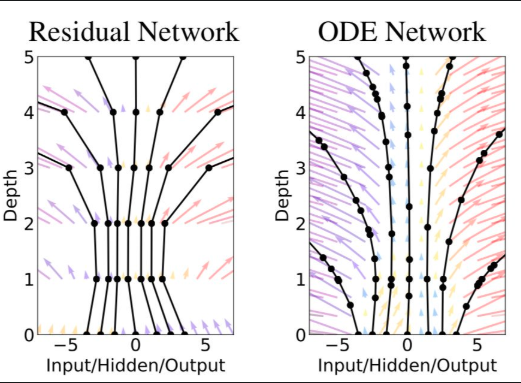
\includegraphics[scale=0.7]{resnetvsodenet.png}
\end{center}

\textbf{voir def vector field}

\textbf{voir probleme du vanishing gradient dans les nn regulier}

\textbf{ recherche the Universal Approximation Theorem states that, for enough layers or enough parameters, $ML(x)$ can approximate any nonlinear function sufficiently close (subject to some constraints).}


\end{document}